\documentclass[footheight=20pt, footsepline, headheight=20pt, headsepline]{scrartcl}
%
\usepackage[utf8]{inputenc} % below are various important packages
\usepackage{lmodern}
\usepackage[T1]{fontenc}
\usepackage[english]{babel}
\usepackage{textcomp} 
\usepackage{amsmath}
\usepackage{mathrsfs}
\usepackage{listings}
\usepackage{latexsym}
\usepackage{amssymb}	
\usepackage{amsfonts}
\usepackage{float}
\usepackage{theorem}
\usepackage{graphicx}
\usepackage{placeins}
\usepackage{scrlayer-scrpage}
\usepackage{xcolor}
\usepackage{setspace}
\usepackage{framed}
\usepackage{hyperref} 
\usepackage{pgf,tikz,pgfplots} % possibility to insert geogebra graphs
\usepackage{mathrsfs}
\pgfplotsset{compat=1.15}\usetikzlibrary{arrows} % part of geogebra package
\usepackage{qrcode} % insert qr codes
\usepackage{multicol}
\usepackage{multirow}
\usepackage{xurl}
\usepackage{tabularx}
\usepackage{enumitem}
\usepackage{float}
\usepackage{colortbl,rotating,booktabs} % required packages for Excel2Latex


% Add to length for wider margins
\addtolength{\textwidth}{3cm} % right to margin
\addtolength{\hoffset}{-1.6cm} % left to margin
\addtolength{\voffset}{-2cm} % to top
\addtolength{\textheight}{6.5cm} % to bottom

% Headers-Footers
\definecolor{gro}{gray}{0.6} % define color
\setkomafont{pagehead}{\normalfont\sffamily} % define header
\setkomafont{pagefoot}{\normalfont\sffamily} % define footer
\addtokomafont{headsepline}{\color{gro}} % define header horizontal line



\renewcommand{\familydefault}{\sfdefault} % font
\linespread{1.2} % increase line spacing

%---------------------------------------------------------------------------
\begin{document} % every document starts with \begin{document}
%\doublespacing
\title{LAB REPORT (Lab-2) \\[1cm] \large{\textbf{CSE 3113: Microprocessor and Assembly Language Lab}}\\[1cm]} 
\author{Jahir Sadik Monon \\ Roll - 32}
\date{\vspace{10cm}  Submitted to, \\[0.5cm] Dr. Upama Kabir \\[0.5cm] Department of Computer Science and Engineering \\[0.5cm] University Of Dhaka}
\maketitle
%---------------------------------------------------------------------------
\newpage
\tableofcontents 
%---------------------------------------------------------------------------
\newpage
\section*{Task - 1}
\addcontentsline{toc}{section}{Task - 1}
\subsection*{Problem Statement}
\addcontentsline{toc}{subsection}{Problem Statement}
This problem is same as the sample problem. W = X + Y + Z. Once again, let X = 9, Y = 8, Z = 5 and I assume that r4 = X, r3 = Y, r2 = Z. In this case, you will put the data in memory in the form of constants before the program runs.
\subsection*{Detail explanation of the code}
\addcontentsline{toc}{subsection}{Detail explanation of the code}
The solution approach to this problem is the same as the sample problem shown in the lab except for the fact that we use the \verb|EQU| instruction to equate names with addresses or data. I have used the instruction,\\ \verb|X  EQU 9|\\ which means using X in the code is equivalent to using the value 9. The solution procedure is,
\begin{itemize}
  \item Store X, Y, Z in r4, r3 \& r2
  \item Store the temporary summation of r4 + r3 to register r1
  \item Add r1 to r2 to find the sum W, store it to r0
\end{itemize}
\subsection*{Screenshot of the state of the system after the code has been loaded}
\addcontentsline{toc}{subsection}{Screenshot of the state of the system after the code has been loaded}
Here we can see that the registers are loaded with random values as the program is only loaded to the system and not executed yet.
\begin{figure}[ht]
    \centering
    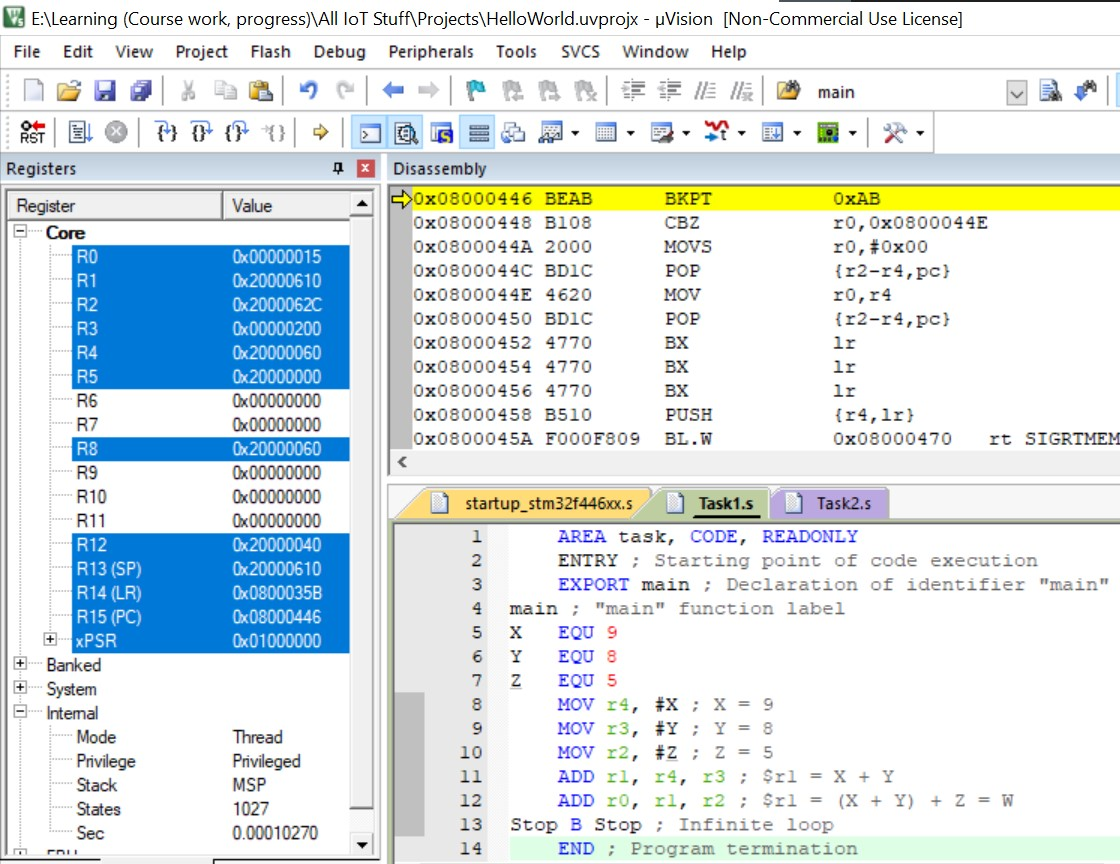
\includegraphics[scale=.8]{images/Task1Before1.jpg}
    \caption{After loading the code on the system}
    \label{fig:before_task_one}
\end{figure}
\FloatBarrier
\subsection*{Screenshot of the state of the system after the code has been executed}
\addcontentsline{toc}{subsection}{Screenshot of the state of the system after the code has been executed}
As we can see, the register value r0 to r4 (the ones that were used in the code) has been changed. r1 holds summation of r3 and r4. r0 holds the summation of r2, r3 \& r4. So finally, the r0 register holds the value of W, which is the summation of registers r4(X), r3(Y) and r2(Z).
\FloatBarrier
\begin{figure}[ht]
    \centering
    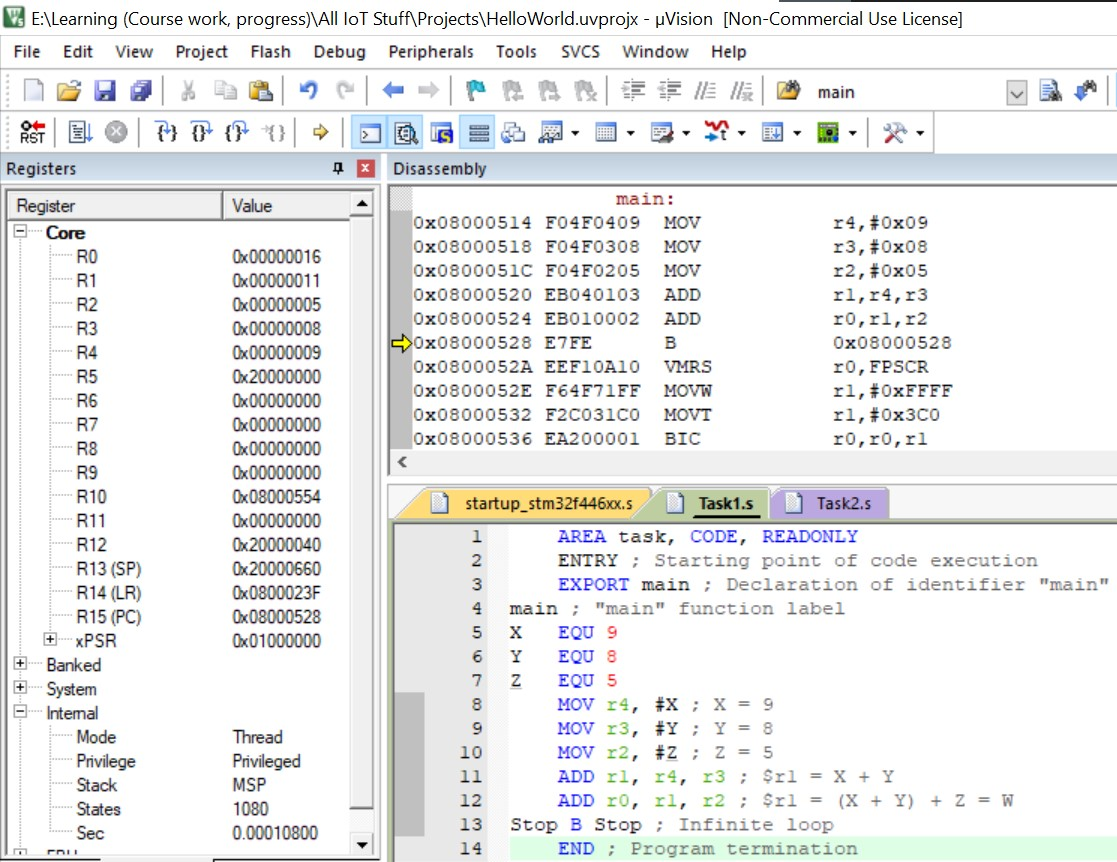
\includegraphics[scale=.8]{images/Task1After1.jpg}
    \caption{After executing the code on the system}
    \label{fig:after_task_one}
\end{figure}


%---------------------------------------------------------------------------
\newpage
\FloatBarrier
\section*{Task - 2}
\addcontentsline{toc}{section}{Task - 2}
\subsection*{Problem Statement}
\addcontentsline{toc}{subsection}{Problem Statement}
Repeat the previous problem once again is W = X + Y + Z Once again, let X = 9, Y = 8, Z = 5 and I assume that r4 = X, r3 = Y, r2 = Z.. In this case, you will put the data in memory as constants before the program runs. But you first use the load register, LDR r4,X instruction to load register r4 with the contents of
memory location r4.
\subsection*{Detail explanation of the code}
\addcontentsline{toc}{subsection}{Detail explanation of the code}
The solution approach to this problem is a little different from the above problem as we have to use the \verb|DCD| instruction to allocate and initialize memory data. We reserve space for X, Y, and Z. In each case we use a DCD assembler directive to reserve a word location (4 bytes) and to initialize it. For example,\\
\verb|X DCD 9 ; create variable X with initial value 9|\\
means ‘call the current line X and store the word 0x00000009 at that location. The instruction \\
\verb|LDR r4, X| \\
Loads the data stored in memory location X in register r4. We do the same load operation for the rest two values.
The rest of the solution procedure is the same as the first task after this point.
\subsection*{Screenshot of the state of the system after the code has been loaded}
\addcontentsline{toc}{subsection}{Screenshot of the state of the system after the code has been loaded}
\begin{figure}[ht]
    \centering
    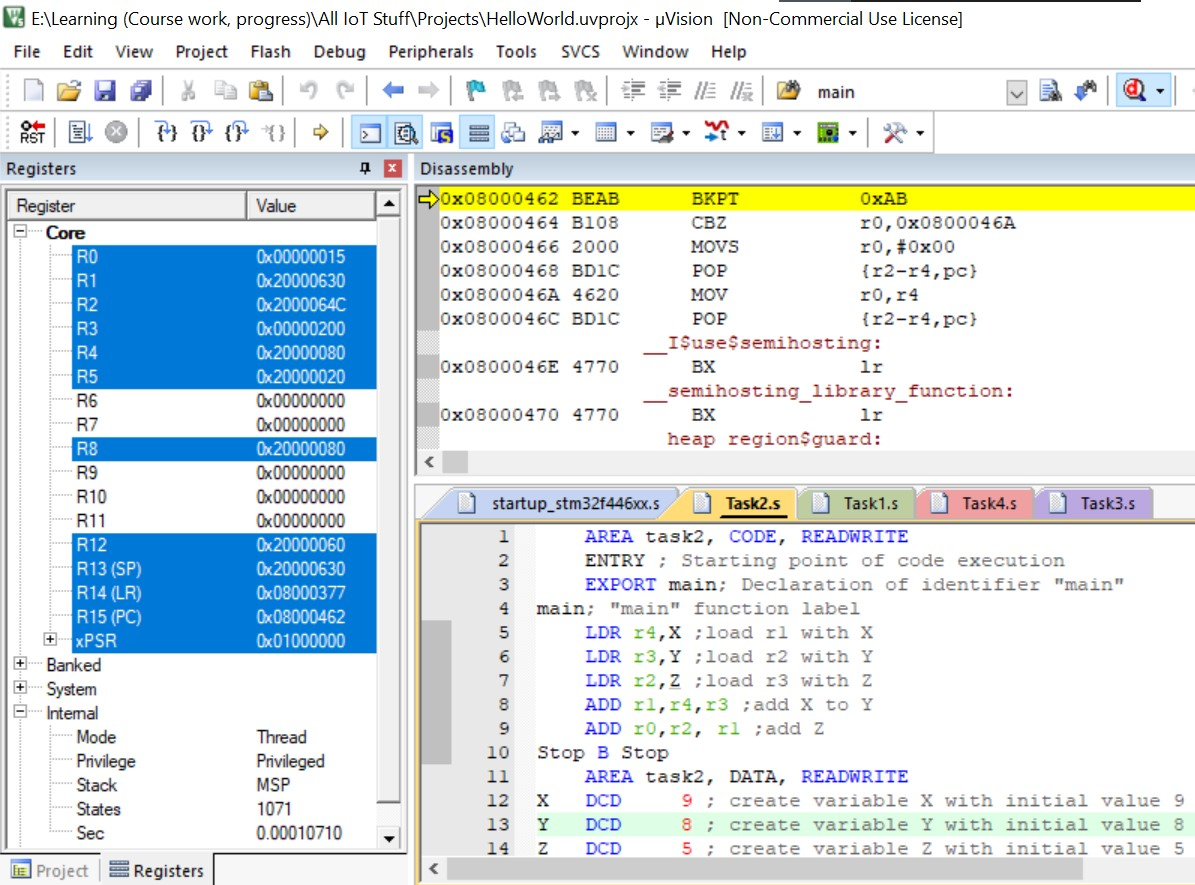
\includegraphics[scale=.75]{images/Task2Before1.jpg}
    \caption{After loading the code on the system}
    \label{fig:before_task_two}
\end{figure}
Here we can see that the registers are loaded with random values as the program is only loaded to the system and not executed yet. 
\FloatBarrier
\begin{figure}[ht]
    \centering
    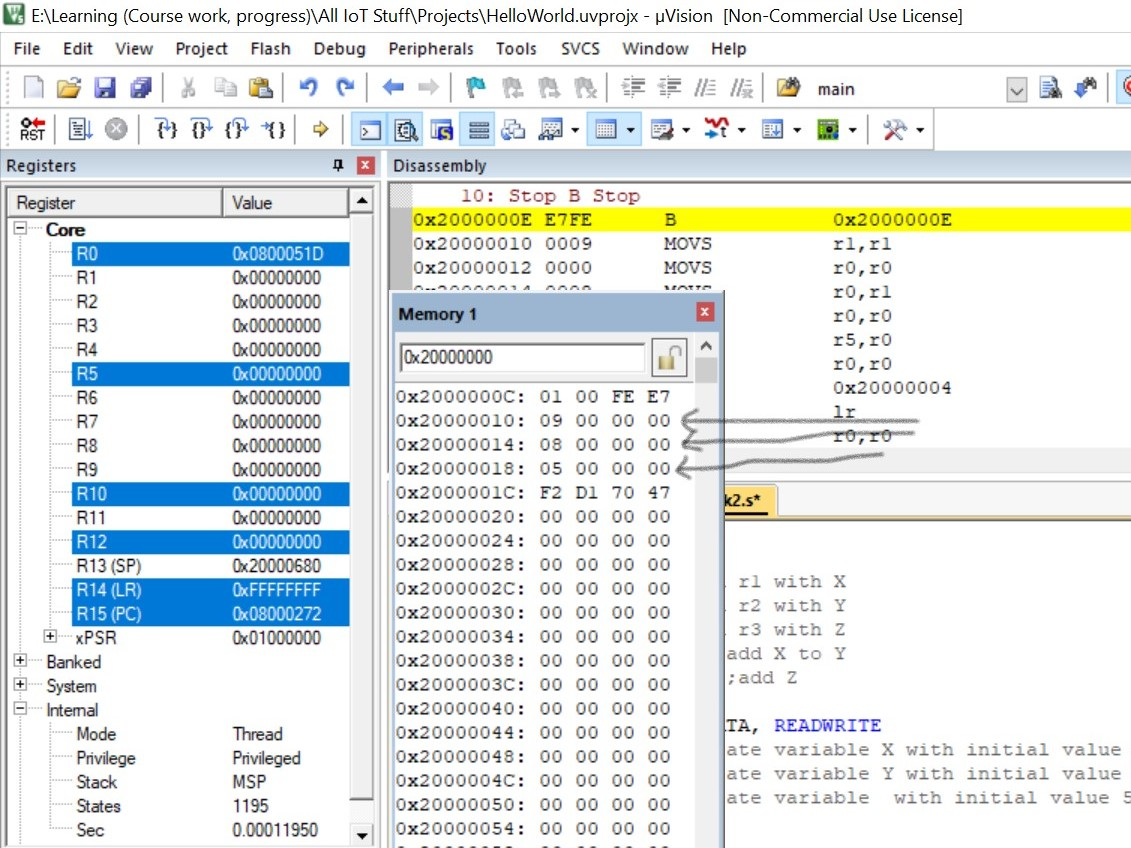
\includegraphics[scale=.75]{images/Task2Before2.jpg}
    \caption{Memory values after loading the code on the system}
    \label{fig:before_task_two_mem}
\end{figure}
\FloatBarrier
As we can see, the memory address from 0x20000010 to 0x2000001C holds the values 9, 8 and 5 before the execution of the code. We then load it on registers while running the code and add it afterwards.
\subsection*{Screenshot of the state of the system after the code has been executed}
\addcontentsline{toc}{subsection}{Screenshot of the state of the system after the code has been executed}
\begin{figure}[ht]
    \centering
    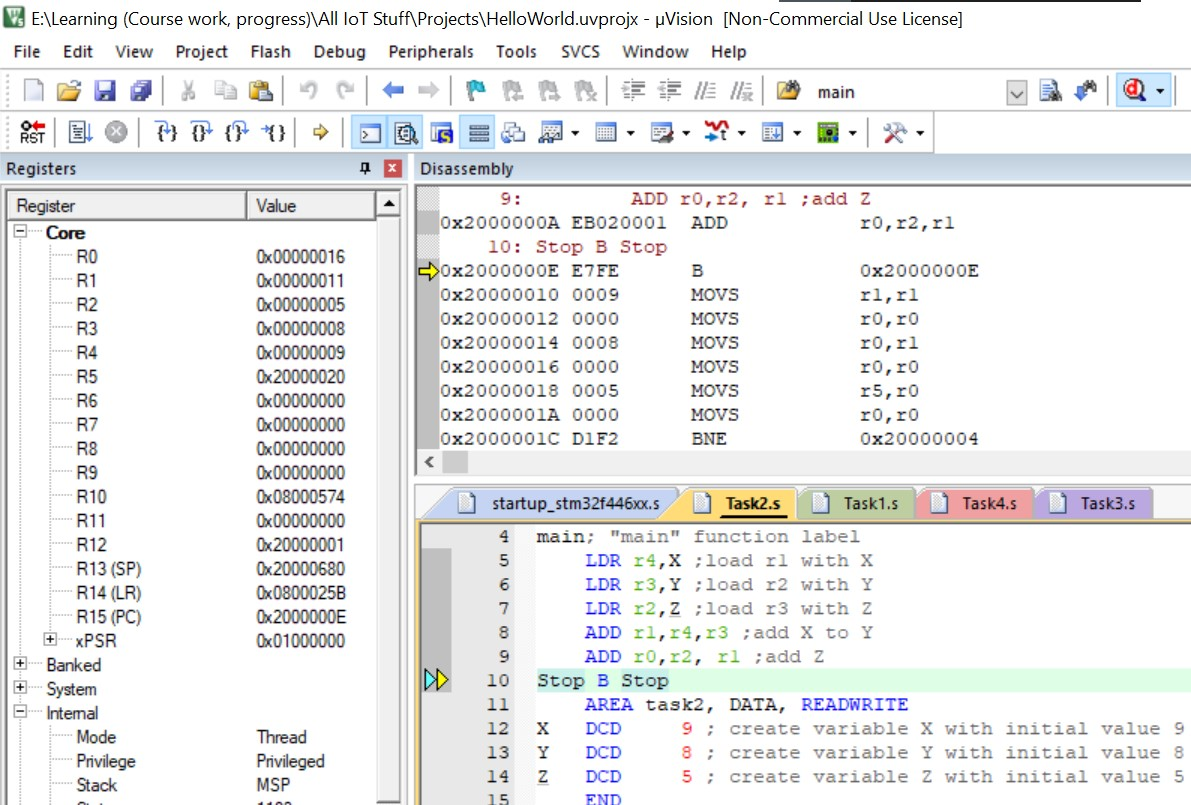
\includegraphics[scale=.75]{images/Task2After1.jpg}
    \caption{After executing the code on the system}
    \label{fig:after_task_two}
\end{figure}
\FloatBarrier
As we can see, the register value r0 to r4 (the ones that were used in the code) has been changed. r1 holds summation of r3 and r4. r0 holds the summation of r2, r3 \& r4. So finally, the r0 register holds the value of W, which is the summation of registers r4(X), r3(Y) and r2(Z).

%---------------------------------------------------------------------------
\newpage
\FloatBarrier
\section*{Task - 3}
\addcontentsline{toc}{section}{Task - 3}
\subsection*{Problem Statement}
\addcontentsline{toc}{subsection}{Problem Statement}
Find the addition of two 16 bit variables v1 and v2.
\subsection*{Detail explanation of the code}
\addcontentsline{toc}{subsection}{Detail explanation of the code}
We want to add to 16-bit numbers in this problem, so we cannot allow a register to load more than 16 bits. So for our problem I have,
\begin{itemize}
    \item Used \verb|MOVW rn, #imm16| instruction to only allow loading 16-bit immediate field values in the registers.
    \item Added the numbers and stored the result in both r1 register and r0 registers so that I can show the difference made in the last step.
    \item In the last step, loaded upper 16-bit field of r0 with 0 to make sure the addition result is rounded to 16-bit value using \verb|MOVT r0, #0|.
\end{itemize}
\subsection*{Screenshot of the state of the system after the code has been loaded}
\addcontentsline{toc}{subsection}{Screenshot of the state of the system after the code has been loaded}
\begin{figure}[ht]
    \centering
    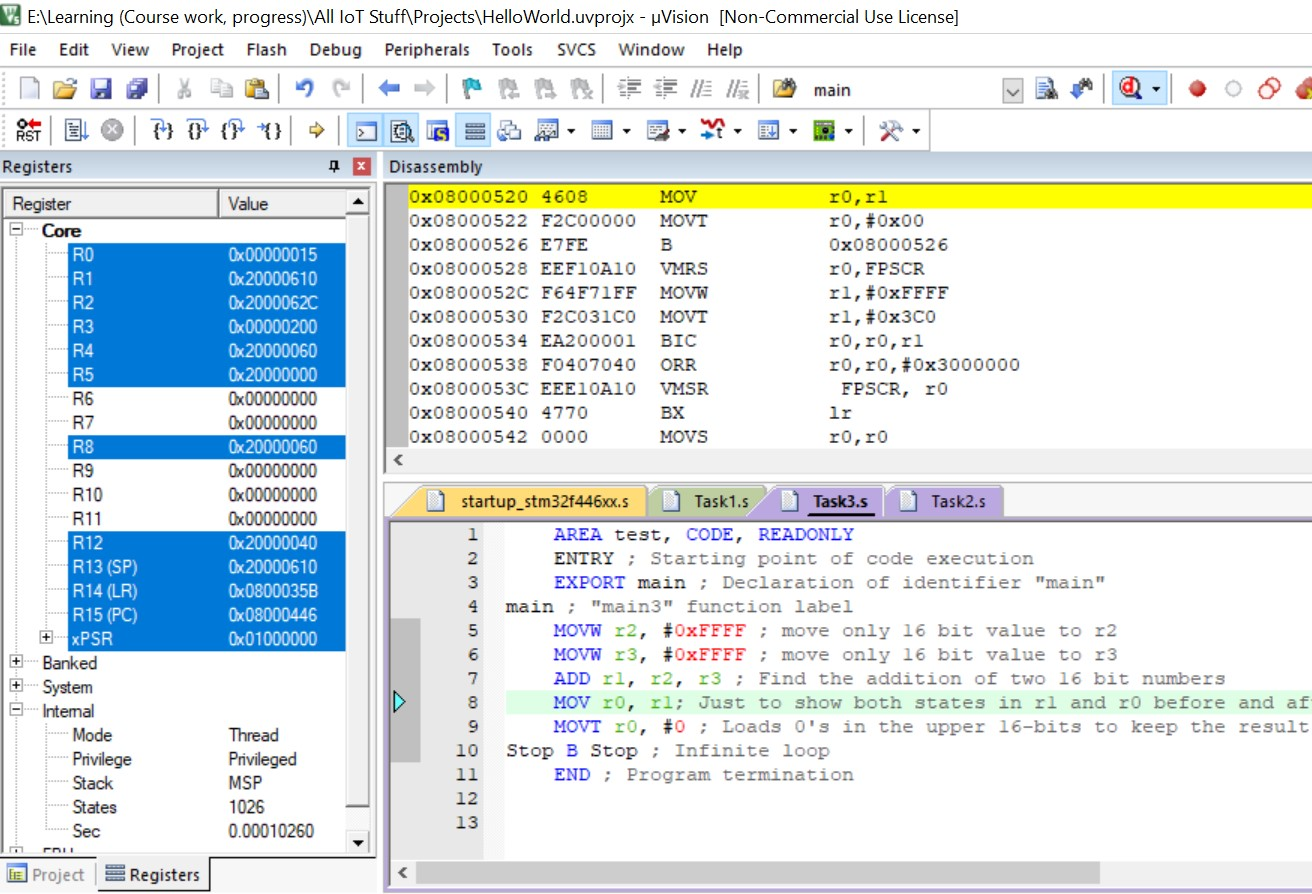
\includegraphics[scale=.75]{images/Task3Before1.jpg}
    \caption{After loading the code on the system}
    \label{fig:before_task_three}
\end{figure}
\FloatBarrier
Here we can see that the registers are loaded with random values as the program is only loaded to the system and not executed yet. 
\subsection*{Screenshot of the state of the system after the code has been executed}
\addcontentsline{toc}{subsection}{Screenshot of the state of the system after the code has been executed}
\begin{figure}[ht]
    \centering
    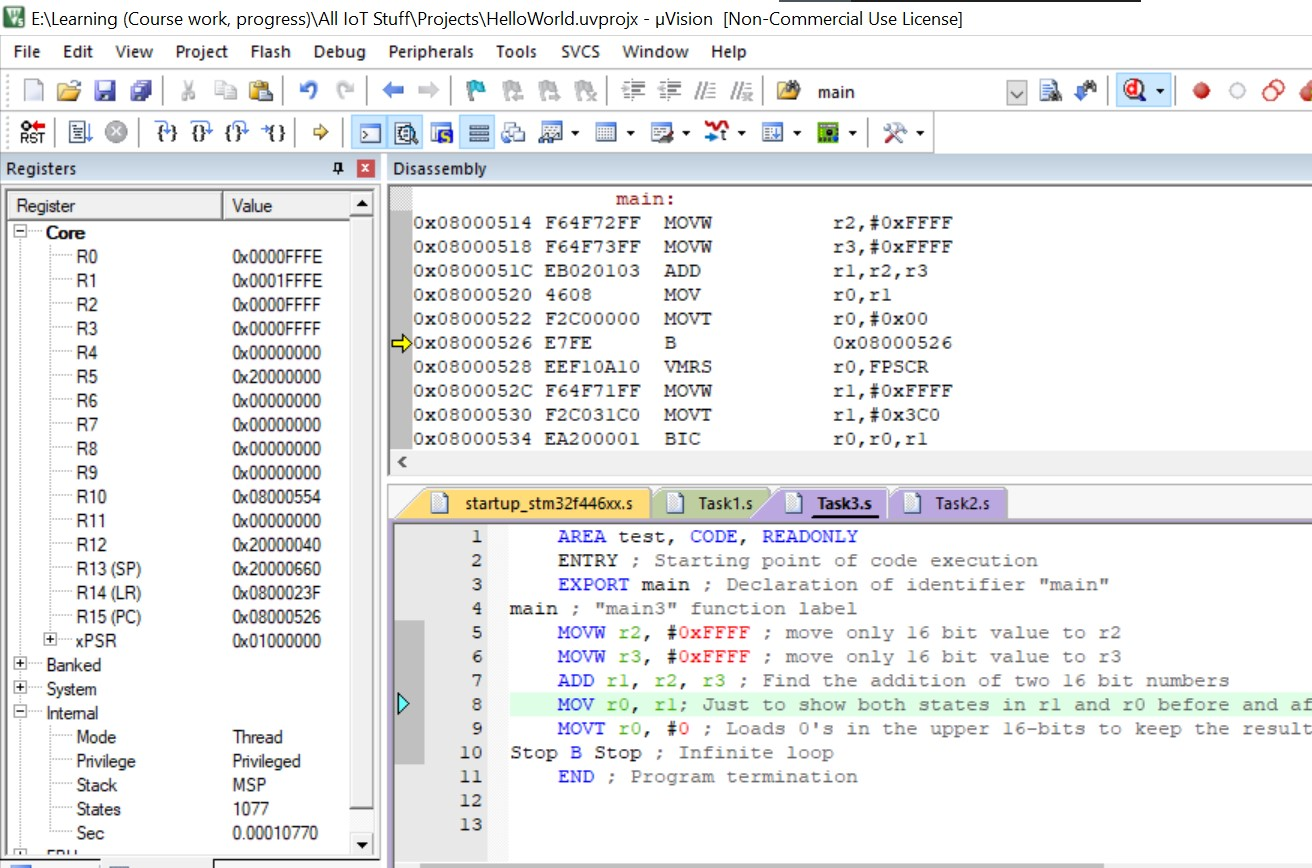
\includegraphics[scale=.75]{images/Task3After1.jpg}
    \caption{After executing the code on the system}
    \label{fig:after_task_three}
\end{figure}
\FloatBarrier
Here we can see that, the two 16-bit values in register r2 and r3 are added and the sum is stored in register r1. I also load the result in r1 in register r0. Then I use \verb|MOVT r0, #0| instruction to load the upper 16-bits of register r0 with 0 values because I only want the last 16-bits of r0, as we're doing addition of 16-bit numbers and want to result to be 16 bit numbers. We can see the 17th bit in register r1 is 1 as overflow occured in our example, but no 17th bit 1 in present in r0 because we loaded 0's in upper 16-bits to round it.

%---------------------------------------------------------------------------

\newpage
\FloatBarrier
\section*{Task - 4}
\addcontentsline{toc}{section}{Task - 4}
\subsection*{Problem Statement}
\addcontentsline{toc}{subsection}{Problem Statement}
Find the smaller of two integer numbers.
\subsection*{Detail explanation of the code}
\addcontentsline{toc}{subsection}{Detail explanation of the code}
I needed conditional logic to complete this task. I loaded r0 and r1 with values 7 and 5 respectively(random values). Then I stored the smaller of the two numbers in the register r2. To accomplish this,
\begin{itemize}
  \item Store 7 in r1, and 5 in r0. Any Two integers can be taken in this case.
  \item Compare r1 and r0 using \verb|CMP r1, r0|
  \item The comparison operation changes the flag values.
  \item I have used condition suffix LT(less than) and GE(greater than or equals) to specify that I want that statement to run only in case that condition suffices.
  \item Finally, I have moved only the smaller value to register r2 using conditional statement.
  \item If two values are same, we can put either one of them in register r2.
\end{itemize}
\FloatBarrier
\subsection*{Screenshot of the state of the system after the code has been loaded}
\addcontentsline{toc}{subsection}{Screenshot of the state of the system after the code has been loaded}
\begin{figure}[ht]
    \centering
    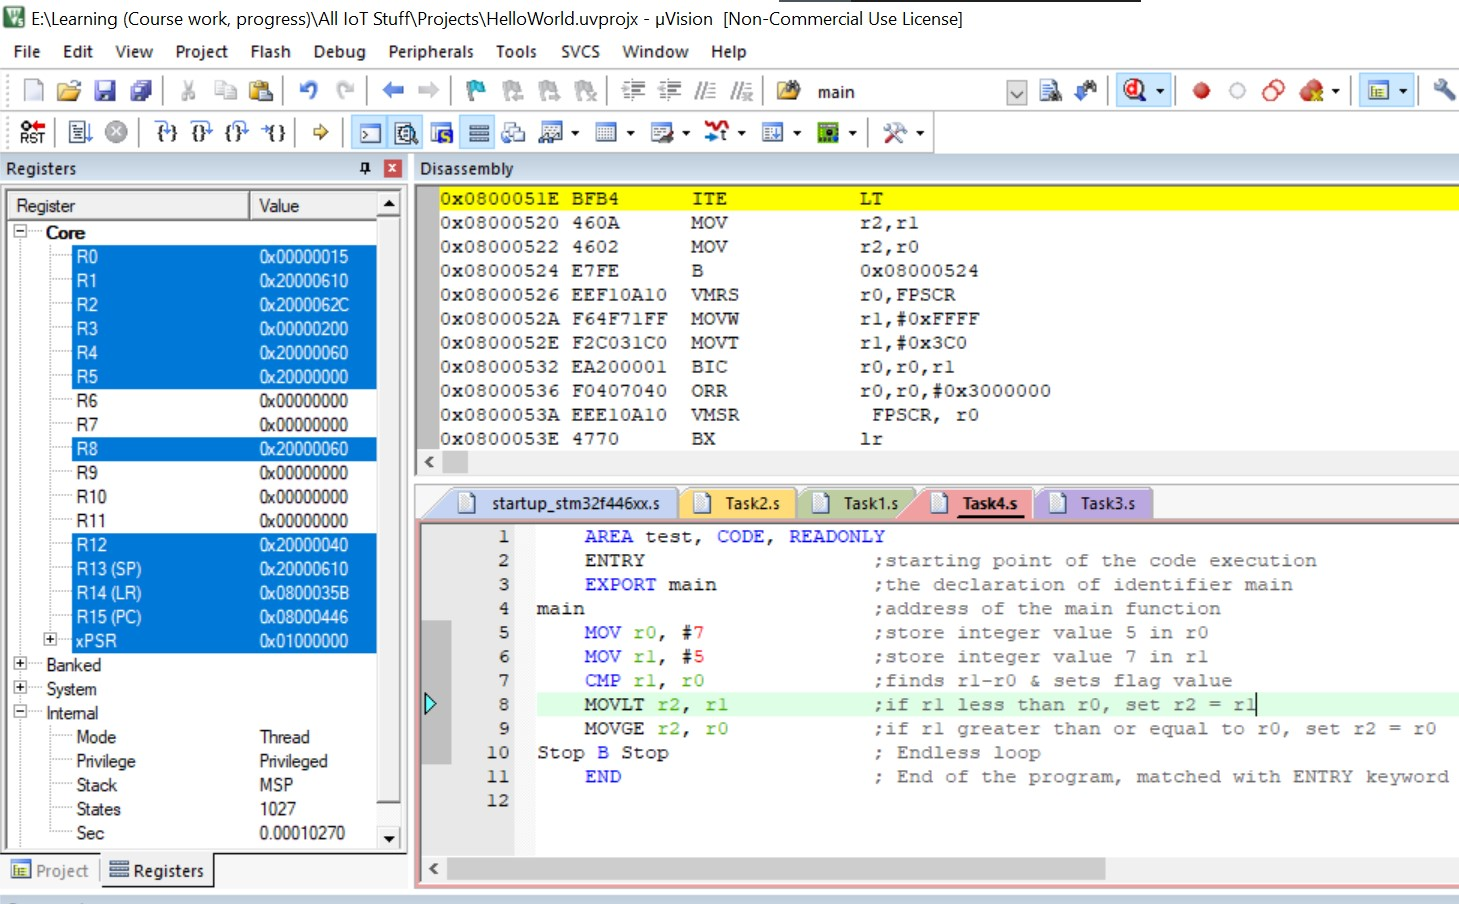
\includegraphics[scale=.7]{images/Task4Before1.jpg}
    \caption{After loading the code on the system}
    \label{fig:before_task_four}
\end{figure}
\FloatBarrier
Here we can see that the registers are loaded with random values as the program is only loaded to the system and not executed yet.
\subsection*{Screenshot of the state of the system after the code has been executed}
\addcontentsline{toc}{subsection}{Screenshot of the state of the system after the code has been executed}
\begin{figure}[ht]
    \centering
    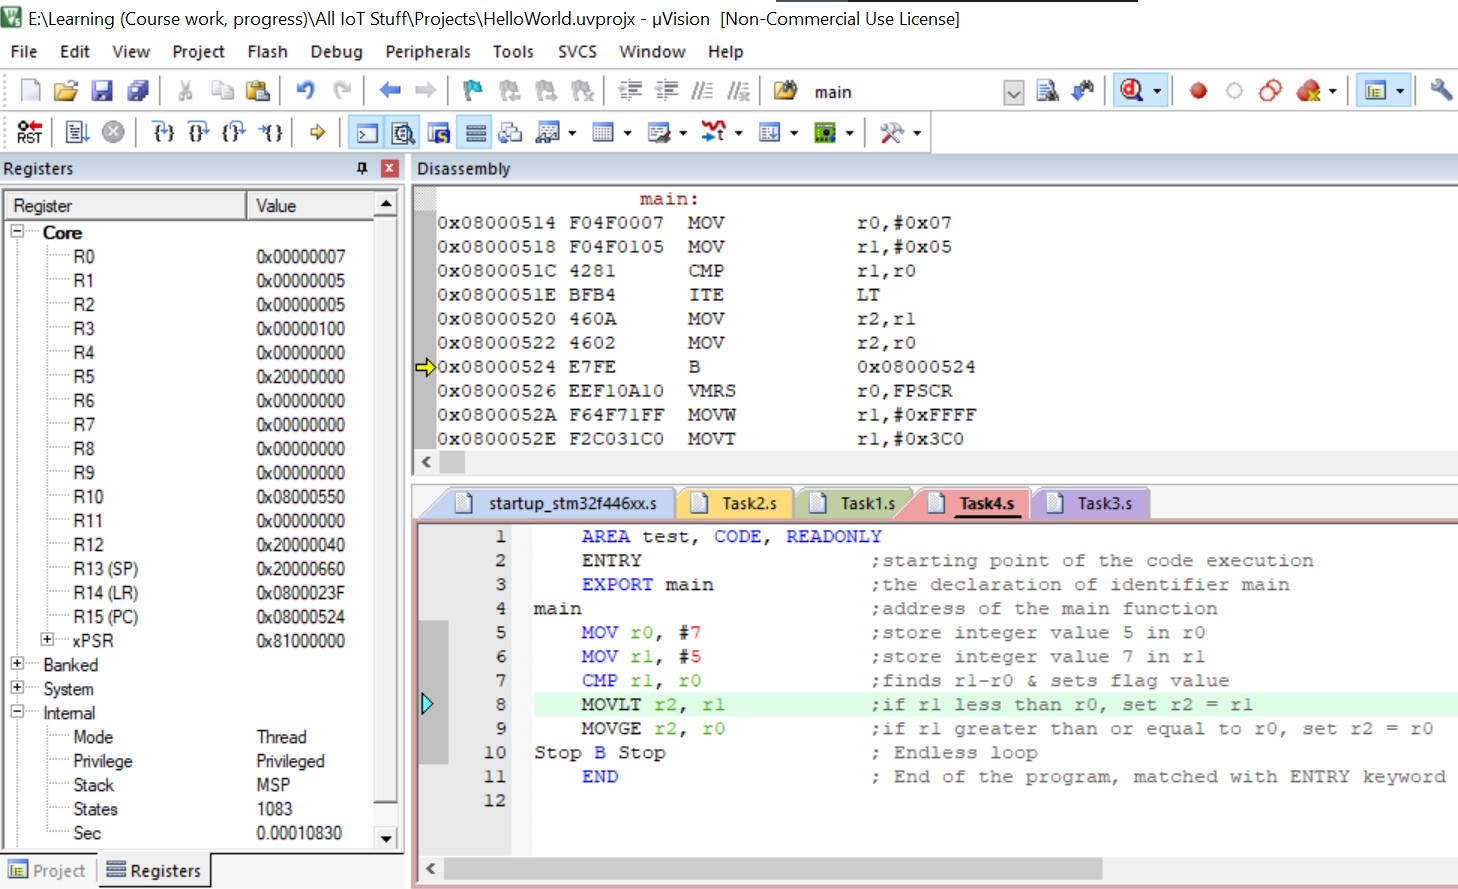
\includegraphics[scale=.7]{images/Task4After1.jpg}
    \caption{After executing the code on the system}
    \label{fig:after_task_four}
\end{figure}
\FloatBarrier
As we can see from the screenshot of register values after execution of the code, the r2 register holds the smaller value after comparison and conditional operation.
\end{document}
